\let\negmedspace\undefined
\let\negthickspace\undefined
\documentclass[journal]{IEEEtran}
\usepackage[a5paper, margin=10mm, onecolumn]{geometry}
\usepackage{tfrupee} % Include tfrupee package

\setlength{\headheight}{1cm} % Set the height of the header box
\setlength{\headsep}{0mm}     % Set the distance between the header box and the top of the text

\usepackage{gvv-book}
\usepackage{gvv}
\usepackage{cite}
\usepackage{amsmath,amssymb,amsfonts,amsthm}
\usepackage{algorithmic}
\usepackage{graphicx}
\usepackage{textcomp}
\usepackage{xcolor}
\usepackage{txfonts}
\usepackage{listings}
\usepackage{enumitem}
\usepackage{mathtools}
\usepackage{gensymb}
\usepackage{comment}
\usepackage[breaklinks=true]{hyperref}
\usepackage{tkz-euclide} 
\usepackage{listings}
\usepackage[latin1]{inputenc}                                
\usepackage{color}                                            
\usepackage{array}                                            
\usepackage{longtable}                                       
\usepackage{calc}                                             
\usepackage{multirow}                                         
\usepackage{hhline}                                           
\usepackage{ifthen}                                           
\usepackage{lscape}

\begin{document}

\bibliographystyle{IEEEtran}
\vspace{3cm}

\title{12.6.6.17}
\author{EE24BTECH11011 - Pranay Kumar}
{\let\newpage\relax\maketitle}

\renewcommand{\thefigure}{\theenumi}
\renewcommand{\thetable}{\theenumi}
\setlength{\intextsep}{10pt} % Space between text and floats

\numberwithin{equation}{enumi}
\numberwithin{figure}{enumi}
\renewcommand{\thetable}{\theenumi}

\textbf{QUESTION} : \\
Show that the height of the cylinder of maximum volume that can be inscribed in a sphere of radius $R$ is $\frac{2R}{\sqrt{3}}$. Also, find the maximum volume.\\

\textbf{SOLUTION} : \\

\textbf{Theoretical solution} : \\
Let the height of the cylinder be $h$ and the radius of the cylinder base be $r$. From the geometry of the problem, the relationship between $h$, $r$, and $R$ is:
\begin{align}
    r^2 + \left(\frac{h}{2}\right)^2 &= R^2 \label{eq:geometry}
\end{align}

The volume of the cylinder is:
\begin{align}
    V &= \pi r^2 h
\end{align}

Substituting $r^2$ , we get:
\begin{align}
    V(h) &= \pi \left(R^2 - \frac{h^2}{4}\right) h \label{eq:volume}
\end{align}

To maximize $V(h)$, we differentiate with respect to $h$:
\begin{align}
    \frac{dV}{dh} &= \pi \left( R^2 - \frac{3h^2}{4} \right) \label{eq:dv}
\end{align}

Setting $\frac{dV}{dh} = 0$, we get:
\begin{align}
    R^2 - \frac{3h^2}{4} &= 0 \\
    h &= \frac{2R}{\sqrt{3}}
\end{align}

Substituting $h = \frac{2R}{\sqrt{3}}$ into  the maximum volume is:
\begin{align}
    V_{\text{max}} &= \frac{2\pi R^3}{3\sqrt{3}}
\end{align}

\textbf{Computational solution} : \\

Finding the maximum volume can also be done using the \textbf{Gradient Ascent method}. The iterative update rule is:
\begin{align}
    h_{n+1} &= h_n + \alpha \frac{dV}{dh}\Big|_{h=h_n}
\end{align}
where $\alpha$ is the learning rate. we have:
\begin{align}
    h_{n+1} &= h_n + \alpha \pi \left( R^2 - \frac{3h_n^2}{4} \right)
\end{align}

Taking:
\begin{align}
    \alpha &= 0.001 \\
    h_0 &= 1
\end{align}
we find:
\begin{align}
    h_{\text{max}} &= 1.1547 \quad (\text{approximates } \frac{2R}{\sqrt{3}}) \\
    V_{\text{max}} &= 2.418 \quad (\text{approximates } \frac{2\pi R^3}{3\sqrt{3}})
\end{align}

\begin{figure}[h]
\centering
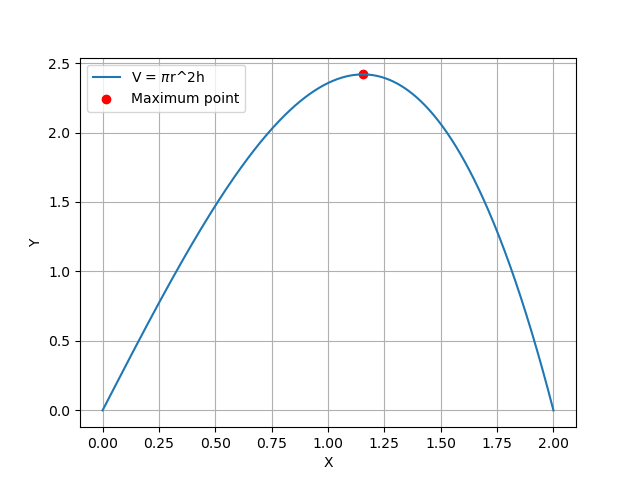
\includegraphics[width=\columnwidth]{figs/fig.png}
\label{fig:Plot1} 
\end{figure}

\end{document}

